% \appendix

\chapter{Appendix: Signal Strength and Path Loss Visualization}

\section{Overview}
This appendix introduces practical visualization of signal strength decay over distance using:
\begin{itemize}
  \item Free Space Path Loss (FSPL)
  \item Log-distance Path Loss model
\end{itemize}

\section{Simulation}
We provide both a Jupyter notebook and an interactive Streamlit app for hands-on exploration.

%\#✅ LaTeX Code to Embed FSPL Plot\#

\begin{figure}[H]
    \centering
    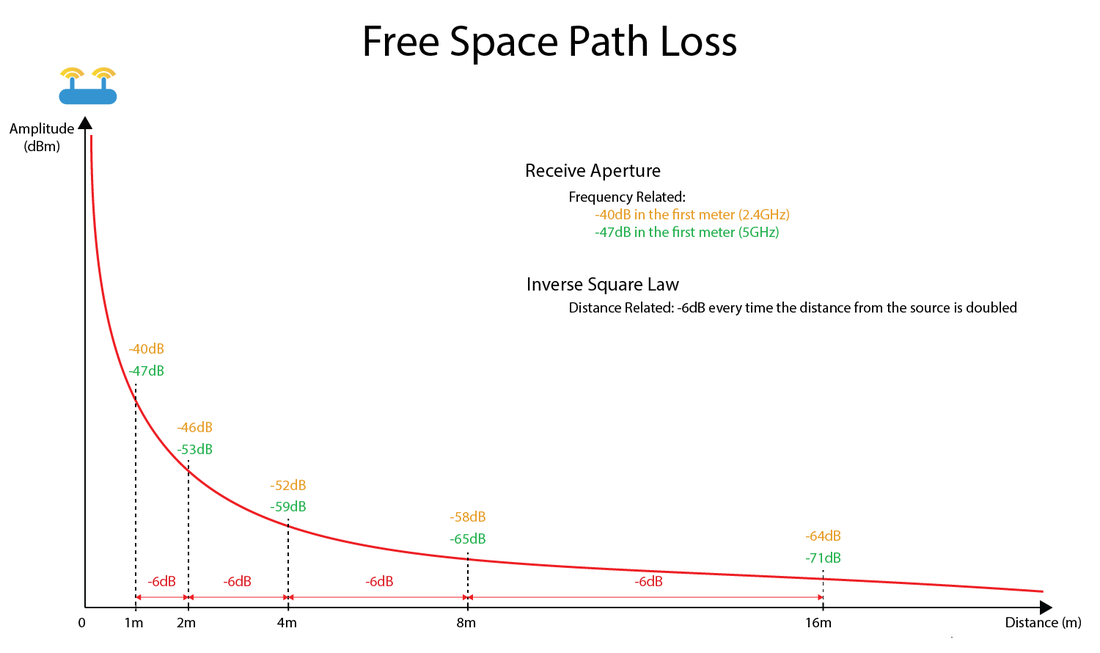
\includegraphics[width=0.85\textwidth]{./figures/fspl_plot.png}
    \caption{Free Space and Log-distance Path Loss vs. Distance}
    \label{fig:fspl_log_loss}
\end{figure}

\subsection{Notebook}
The notebook visualizes path loss vs. distance.

\textbf{Download:}
\begin{itemize}
  \item \href{run:./notebooks/A1-signal_strength.ipynb}{Jupyter Notebook (A1)}
  \item \href{run:./figures/fspl_plot.png}{Generated Path Loss Plot}
\end{itemize}

\subsection{Interactive Streamlit App}
The following app allows real-time manipulation of key parameters:
\begin{itemize}
  \item Frequency (GHz)
  \item Maximum Distance
  \item Path Loss Exponent
\end{itemize}

\textbf{Link:} \href{http://<your-deployed-url>:8501}{Open Signal Visualizer App}

\section{References}
\begin{enumerate}
  \item Rappaport, T. S. (2014). \textit{Wireless Communications: Principles and Practice}.
  \item 3GPP Technical Specification TS 36.942.
  \item Fundamentals of 5G Mobile Networks – Wiley.
\end{enumerate}
